%
% Portuguese-BR version
%

\documentclass{report}

\usepackage{ipprocess}
% Use longtable if you want big tables to split over multiple pages.
\usepackage{longtable}
\usepackage[utf8]{inputenc} 
\usepackage[brazil]{babel} % Uncomment for portuguese
\usepackage{pdflscape} % set ladscape/portrait pdf pages
\usepackage{tikz}
\usepackage{tikz-uml}
\usepackage{multirow}
\usepackage{graphicx}

\sloppy

\graphicspath{{./pictures/}} % Pictures dir
\makeindex
\begin{document}


%%%%%%%%%%%%%%%%%%%%%%%%%%%%%%%%%%%%%%%%%%%%%%%%%%
%% Building front cover
%%%%%%%%%%%%%%%%%%%%%%%%%%%%%%%%%%%%%%%%%%%%%%%%%%
\DocumentTitle{Documento de Arquitetura}
\Project{MUSA}
\Organization{Fazemos Qualquer Negócio Inc.}
\Version{Compilação 3.1}
% Make front cover
\capa
%

%%%%%%%%%%%%%%%%%%%%%%%%%%%%%%%%%%%%%%%%%%%%%%%%%%
%% Revision History
%%%%%%%%%%%%%%%%%%%%%%%%%%%%%%%%%%%%%%%%%%%%%%%%%%
\section*{\center Histórico de Revisões}
	\vspace*{1cm}
	\begin{table}[h!]
		\centering
		\begin{longtable}[pos]{|m{2cm} | m{7.2cm} | m{3.8cm}|} \hline \cellcolor[gray]{0.9}

\textbf{Data} & \cellcolor[gray]{0.9}\textbf{Descrição} & \cellcolor[gray]{0.9} \textbf{Autor(es)}\\ \hline
      \small 25/06/2014 & \small Concepção do documento & \small joaocarlos \\ \hline
      \small 15/10/2014 & \small Adição da subseção de acesso à memória & \small weversongomes \\ \hline
      \small 16/10/2014 & \small Adição da seção "Leitura da Instrução" e modificação do nome do projeto. & \small santana22 e gabri14el.\\ \hline
      \small 19/10/2014 & \small Modificações na seção "Leitura da Instrução" & \small santana22 \\ \hline
      \small 20/10/2014 & \small Correções na subseção de acesso à memória & \small weversongomes \\ \hline
      \small 25/10/2014 & \small Adição das descrições da codificação & \small manuellemacedo \\ \hline
      \small 29/10/2014 & \small Unificação das subseções de acesso à memória com a de write back & \small weversongomes \\ \hline
      \small 29/10/2014 & \small Adição das descrições dos componentes & \small manuellemacedo \\ \hline
      \small 30/10/2014 & \small Adição do Datapath (Instruction Fetch) & \small santana22 e gabri14el \\ \hline
      \small 30/10/2014 & \small Alterações na subseção de acesso à memória com definições de número de bits & \small weversongomes \\ \hline
      \small 03/11/2014 & \small Correções na subseção "Leitura da Instrução" & \small weversongomes \\ \hline
      \small 05/11/2014 & \small Modificação dos datapaths internos & \small tarleswalker \\ \hline
      \small 05/11/2014 & \small Alteração nos opcodes & \small manuellemacedo \\ \hline
      \small 27/11/2014 & \small Refatoração da introdução e codificação & \small manuellemacedo \\ \hline
      \small 06/12/2014 & \small Atualização das informações do Instruction Fetch & \small santana22 \\ \hline
      \small 10/12/2014 & \small Atualização da tabela de microinstruções  & \small mirelarios \\ \hline
      \small 10/12/2014 & \small Modificando as informações contidas nos diagramas de classe de cada estágio  & \small  santana22 \\ \hline
      \small 11/12/2014 & \small Refatoração da introdução e codificação & \small manuellemacedo \\ \hline
      \small 11/12/2014 & \small Alteração no datapath do Intruction Fetch  & \small mirelarios \\ \hline
      \small 14/12/2014 & \small Atualização dos diagramas de classe & \small santana22 \\ \hline
	\end{longtable}
	\end{table}

% TOC instantiation
\tableofcontents

%%%%%%%%%%%%%%%%%%%%%%%%%%%%%%%%%%%%%%%%%%%%%%%%%%
%% Document main content
%%%%%%%%%%%%%%%%%%%%%%%%%%%%%%%%%%%%%%%%%%%%%%%%%%
\chapter{Introdução}
  
	\section{Introdução}

 A \textbf{Fazemos Qualquer Negócio Inc.} foi contratada para o desenvolvimento do \textit{IP-Core} \textbf{MUSA}, que é um micro processador de
 propósito geral que será utilizado em escolas de países africanos com o intuito de impulsionar o desenvolvimento deste continente. As seções
 subsequentes apresentam os requisitos funcionais e não funcionais como parte da fase de \textbf{Concepção} do IP-process.
 Os requisitos listados foram definidos a partir das necessidades do cliente para produção do \textit{MUSA}.

\chapter{Visão Geral da Arquitetura}

%	\section{Restrições}
	\begin{itemize}
	\item \textbf{Restrições --} %fazer junto com os desenvolvedores
	\end{itemize}
	
	\section{Codificação das instruções}
	Instrução é uma palavra da linguagem de máquina, sua codificação é de fundamental importância para o processamento das operações.	Todas as instruções contém 32 bits. Exitem 4 formatos de instruções: R (R-type), I (I-type), Load/Store e Jump. Os OPCODES são os códigos de operação da instrução, neste documento ele é representação em números hexadecimais.\\
	
  \FloatBarrier
    \begin{center}
\begin{longtable}[pos]{| c | c | c | m{7cm} |} \hline    
          \multicolumn{1}{|c|}{\cellcolor[gray]{0.9}\textbf{Formato da instrução}} & 
          \multicolumn{1}{c|}{\cellcolor[gray]{0.9}\textbf{Instrução}} & 
          \multicolumn{1}{c|}{\cellcolor[gray]{0.9}\textbf{Descrição}} \\ \hline
          \endfirsthead
          \hline
          \multicolumn{3}{|l|}
          {{\bfseries continuação da página anterior}} \\
          \hline
          \multicolumn{1}{|c|}{\cellcolor[gray]{0.9}\textbf{Formato da Instrução}} & 
          \multicolumn{1}{c|}{\cellcolor[gray]{0.9}\textbf{Instrução}} & 
          \multicolumn{1}{c|}{\cellcolor[gray]{0.9}\textbf{Descrição}} \\ \hline
          \endhead

          \multicolumn{3}{|r|}{{continua na próxima página}} \\ \hline
          \endfoot

          \hline
          \endlastfoot 
           
			\multirow{8}{*}{R-type} & ADD & Soma dois valores \\ \cline{2-3}	
	& SUB & Subtrai dois valores \\ \cline{2-3}	
	& MUL & Multiplica dois valores \\ \cline{2-3}	
	& DIV & Divide dois valores \\ \cline{2-3}
	& AND & AND lógico \\ \cline{2-3}
	& OR & OR lógico  \\ \cline{2-3}
	& CMP & Compara dois valores \\ \cline{2-3}
	& NOT & NOT lógico \\ \hline 
	\multirow{4}{*}{I-type} & ADDI & Soma dois valores,um destes imediato. \\ \cline{2-3}
	& SUBI & Subtrai dois valores, um destes imediato. \\ \cline{2-3}
	& ANDI & AND lógico de dois valores, um destes imediato. \\ \cline{2-3}
	& ORI & OR lógico de dois valores, um destes imediato. \\ \cline{2-3}
	& LW & Leitura de um dado da memória de dados \\ \cline{2-3}
	& SW & Armazena um dado na memória de dados \\ \hline
	\multirow{6}{*}{Jump} & JP & Desvia para um destino \\ \cline{2-3}
	& JPC & Desvia para um destino relativo ao PC \\ \cline{2-3}
	& BRFL & Desvia para um destino se RF==CST \\ \cline{2-3}
	& CALL & Chamada de subrotina \\ \cline{2-3}
	& RET & Retorno de Subrotina \\ \cline{2-3}
	& HALT & Parada do sistema \\ \cline{2-3}
	& NOPE & Refresh no módulo \\ \hline
\end{longtable}
\end{center}


	O formato R está relacionado as instruções lógicas e aritméticas.
	\begin{figure}[H]
    	\centering
    	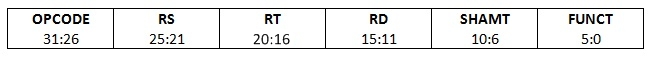
\includegraphics{r-format}
    	\caption{Formato R}
		\label{r_format}
	\end{figure}
	Seus respectivos campos são:
	\begin{itemize}
	\item \textbf{OPCODE} - Código da operação básica da instrução.
	\item \textbf{RS} - Registrador do primeiro operando de origem.
	\item \textbf{RT} - Registrador do segundo operando de origem.
	\item \textbf{RD} - Registrador destino.
	\item \textbf{SHAMT} - \textit{Shift amount}; Quantidade de deslocamento.
	\item \textbf{FUNCT} - Função; Esse campo seleciona a variante específica da operação no campo opcode, e as vezes, é chamado de código de função.
\end{itemize}	

\begin{table}[H]
\centering
	\begin{tabular}{|c|c|c|}
  	\hline 
  	\cellcolor[gray]{0.9}\textbf{OPCODE} & \cellcolor[gray]{0.9}\textbf{INSTRUCTION} & \cellcolor[gray]{0.9}\textbf{FUNCTION} \\ 
  	\hline 
  	0x00 & ADD & 0x20 \\ 
  	\hline 
  	0x00 & SUB & 0x22 \\ 
  	\hline 
  	0x00 & MUL & 0x18 \\ 
  	\hline 
  	0x00 & DIV & 0x1A \\ 
  	\hline 
  	0x00 & AND & 0x24 \\ 
  	\hline 
  	0x00 & OR & 0x25 \\ 
  	\hline 
  	0x00 & CMP & 0x1C \\ 
  	\hline 
  	0x00 & NOT & 0x1D \\ 
  	\hline 
  	\end{tabular} 
  	\caption{Definição dos OPCODES do formato R}
  \end{table} 
  	 	
  	
	 Um segundo tipo de formato de instrução é chamado de formato I, utilizado pelas instruções imediatas e de transferência de dados.
	\begin{figure}[H]
    	\centering
    	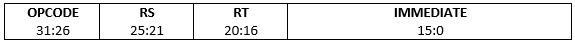
\includegraphics{i-format}
    	\caption{Formato I}
		\label{i_format}
  	\end{figure}
Seus respectivos campos são:
	\begin{itemize}
	\item \textbf{OPCODE} - Código da operação básica da instrução.
	\item \textbf{RS} - Registrador do operando de origem.
	\item \textbf{RT} - Registrador destino.
	\item \textbf{ADDRESS OR IMMEDIATE} - Endereço de memória ou constante numérica.
\end{itemize}	  	

\begin{table}[H]
\centering	
\begin{tabular}{|c|c|}
	\hline 
  	\cellcolor[gray]{0.9}\textbf{OPCODE} & \cellcolor[gray]{0.9}\textbf{INSTRUCTION} \\ 
	\hline 
	0x08 & ADDI \\ %
	\hline 
	0x10 & SUBI \\ %
	\hline 
	0x0c & ANDI \\ %
	\hline 
	0x13 & ORI \\ %
	\hline 
	0x23 & LW \\ %
	\hline 
	0x2b & SW \\ %	
%	0x2a
%0x04
%0x04
	\hline 
	\end{tabular} 
	  	\caption{Definição dos OPCODES do formato I}	
\end{table}	
	
 O formato Jump servem para as instruções de desvio incondicional.  	
   	\begin{figure}[H]
    	\centering
    	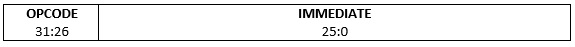
\includegraphics{jump}
    	\caption{Formato Jump}
		\label{jump}
  	\end{figure}
Seus respectivos campos são:
	\begin{itemize}
	\item \textbf{OPCODE} - Código da operação básica da instrução.
	\item \textbf{ADDRESS} - Endereço de memória ou constante numérica.
\end{itemize}
 
\begin{table}[H]
\centering 	
  	\begin{tabular}{|c|c|}
  	\hline 
  	\cellcolor[gray]{0.9}\textbf{OPCODE} & \cellcolor[gray]{0.9}\textbf{INSTRUCTION} \\ 
  	\hline 
  	- & JP \\ 
  	\hline 
  	- & JPC \\ 
  	\hline 
  	0x09 & BRFL \\ 
  	\hline 
  	- & CALL \\ 
  	\hline 
  	- & RET \\ 
  	\hline 
  	- & HALT \\ 
  	\hline 
  	- & NOPE \\ 
  	\hline 
  	\end{tabular} 
  	  	\caption{Definição dos OPCODES do formato Jump}
\end{table}
	
	\section{Descrição dos Componentes}
  A unidade de processamento a ser desenvolvida é composta a partir dos seguintes componentes:

  \begin{itemize}
    \item \textbf{Instruction Fetch --} Módulo responsavel pela busca da instrução na memória de instrução.
    \item \textbf{Instruction Decode e Register Read --} Módulo responsável pela decodificação das instruções e leitura do banco de registradores.
    \item \textbf{Execute Operation or Calculate Address --} Módulo responsável pela execução as operações de caractér lógico/aritmético ou cálculos endereços.
     \item \textbf{Memory Access e Write Back --} Módulo responsável pelo acesso a memória de dados e escrita no banco de registradores.
  \end{itemize}

 % inicio das descrições de arquitetura para cada componente do sistema
\chapter{Descrição da Arquitetura}

	\section{Leitura da Instrução}
	\subsection{Diagrama de Classe}
  \begin{figure}[h!]
    \begin{center}
	\begin{tikzpicture}
	\umlclass[type = control]{Instruction Fetch}{
	+ clock : input bit \\
	+ reset : input bit \\
	+ pcInput : input bit[14] \\ 
	+ pcWrite : input bit \\
	+ pcOutput : output bit[14] \\
	+ instruction : output bit[32] }			
	{
	- \underline{<<comb>> search\_Instruction()} \\
	- <<comb>> next\_PC() 
	}
	\end{tikzpicture}
\end{center}
  \end{figure}
		
		\subsection{Definições de entrada e saída}
		
	\begin{center}
		\begin{longtable}[pos]{| l | c | c | m{7cm} |} \hline
			\multicolumn{1}{|c|}{\cellcolor[gray]{0.9}\textbf{Nome}} & 
			\multicolumn{1}{c|}{\cellcolor[gray]{0.9}\textbf{Tamanho}} & 
			\multicolumn{1}{c|}{\cellcolor[gray]{0.9}\textbf{Direção}} &
			\multicolumn{1}{c|}{\cellcolor[gray]{0.9}\textbf{Descrição}} \\ \hline
			\endhead
			\hline
			\endlastfoot
			clock & 1 & entrada & Clock do sistema \\ \hline
			reset & 1 & entrada & Sinal de reinício do estágio\\ \hline
			pcInput & 32 & entrada & Endereço da instrução a ser buscada \\ \hline
			pcWrite & 1 & entrada & Sinal que habilita a modificação do valor de PC \\ \hline
			push & 1 & entrada & Sinal que habilita a escrita na Pilha de Instruções\\ \hline
			pop & 1 & entrada & Sinal que habilita a leitura da Pilha de Instruções\\ \hline
			pcStack & 32 & saida & Valor do PC armazenado no topo da Pilha de Instruções\\ \hline
			pcOutput & 32 & saída & Endereço da instrução que está sendo executada \\ \hline
			instruction & 32 & saída & Instrução encontrada \\ \hline
			
		\end{longtable}
	\end{center}
	
	%\newpage
	
	\subsection{Datapath Interno}
	\begin{figure}[htpb!]
		\begin{center}
		%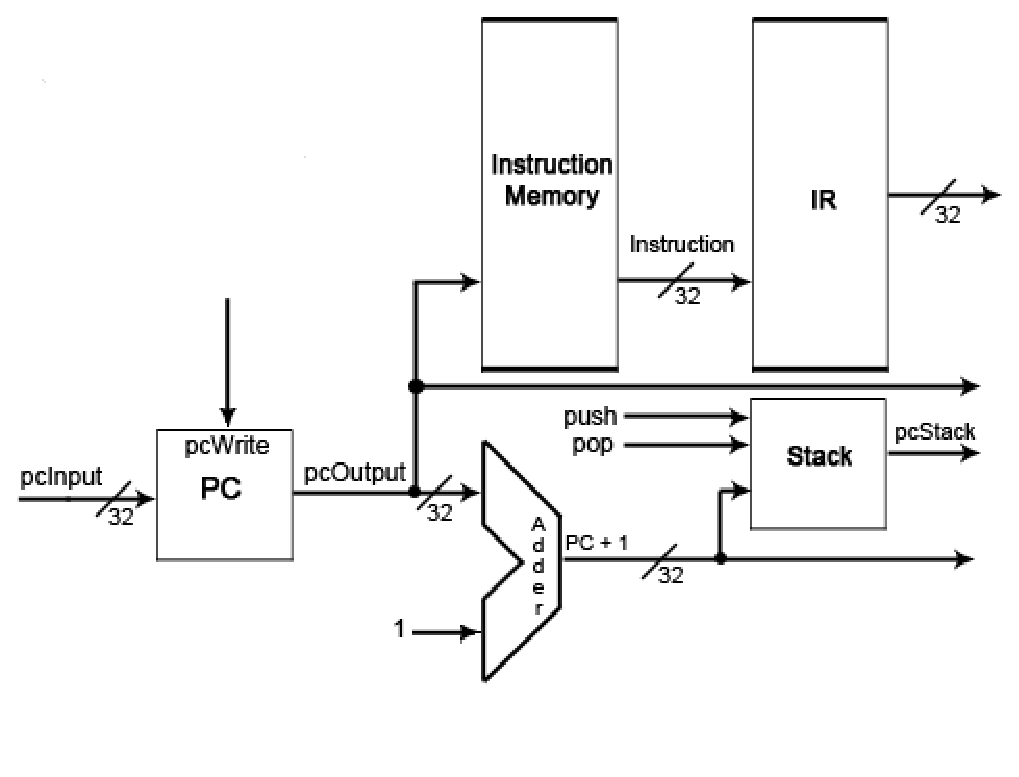
\includegraphics[scale=0.8]{./datapath/step1.eps}
		\end{center}
	\end{figure}
	
	\newpage
	
	\begin{center}
	\begin{tikzpicture}
	\umlclass[x=0,y=0]{Instruction Decode}{
	+ clock : input bit \\
	+ reset : input bit \\
	+ instruction : input bit[32] \\ 
	+ regDst : input bit \\
	+ writeData : input bit \\
	+ writeRegister : input bit \\
	+ word : input bit[16] \\
	+ regDst : output bit \\
	+ branch : output bit \\
	+ memRead : output bit \\
	+ memToReg : output bit \\
	+ aluOp : output bit \\
	+ memWrite : output bit \\
	+ aluSrc : output bit \\
	+ regWrite : output bit \\
	+ jump : output bit \\
	+ readData1 : output bit[32] \\
	+ readData2 : output bit [32] \\
	+ outputWord : output bit [32] \\
	+ registers : reg bit[32] \\}			
	{ % procedures
          - \underline{<<comb>> opcode\_decoder()} \\
          - <<comb>> search\_register() \\
          - <<comb>> set\_write\_register() \\
          - <<sequ>> sign\_extend() \\
          - <<sequ>> zero\_extend()
        }
	\end{tikzpicture}
\end{center}
	\newpage
	
	\section{Estágio de execução}
	\subsection{Diagrama de Classe}
  \begin{figure}[h]
    \begin{center}
	\begin{tikzpicture}
	\umlclass[x=0,y=0]{EX}{
	+ clock : input bit \\
	+ pcInput : input bit[32] \\ 
	+ pcWrite : input bit \\
	+ pcOutput : output bit[32] \\
	+ instruction : output bit[32] \\}			
	{}
	\end{tikzpicture}
\end{center}
  \end{figure}
		
		\subsection{Definições de entrada e saída}
		
	\begin{center}
		\begin{longtable}[pos]{| l | c | c | m{7cm} |} \hline
			\multicolumn{1}{|c|}{\cellcolor[gray]{0.9}\textbf{Nome}} & 
			\multicolumn{1}{c|}{\cellcolor[gray]{0.9}\textbf{Tamanho}} & 
			\multicolumn{1}{c|}{\cellcolor[gray]{0.9}\textbf{Direção}} &
			\multicolumn{1}{c|}{\cellcolor[gray]{0.9}\textbf{Descrição}} \\ \hline
			\endhead
			\hline
			\endlastfoot
			
			data\_a & 32 & Entrada & Dado do primeiro operando. \\ \hline
			data\_b & 32 & Entrada & Dado do segundo operando. \\ \hline
			pc\_in & 32 & Entrada & Valor do PC atual. \\ \hline
			orig\_pc & 2 & Define qual a origem do próximo pc, ou seja, se é branch, jump ou a próxima instrução \\ \hline
			
			
			
			
		\end{longtable}
	\end{center}
	
	\subsection{Datapath Interno}
	
	\begin{figure}[ht]
		\begin{center}
		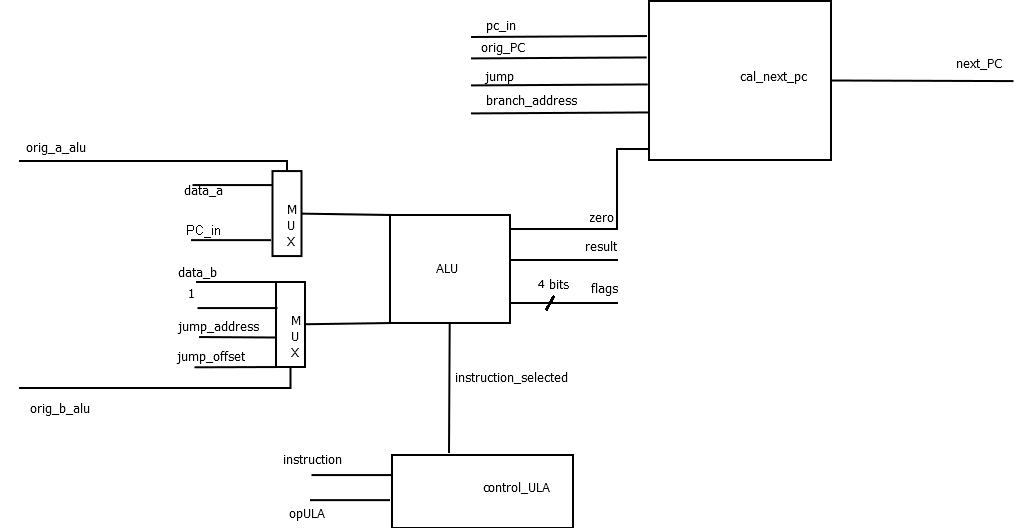
\includegraphics[scale = 0.5]{./datapath/step3.png}
		\caption*{Datapath interno do estágio de execução (EX).}
		\end{center}
	\end{figure}
	
	\newpage
	
	\section{Acesso à memória e write back}
	\subsection{Diagrama de Classe}
  \begin{figure}[H]
    \begin{center}
	\begin{tikzpicture}
	\umlclass[x=0,y=0]{MemoryExecute}{
	+ zero : input bit \\ 
	+ address : input bit \\ 
	+ writeData : input bit[13] \\ 
	+ memRead : input bit \\ 
	+ memWrite : input bit\\ 
	- writeBack : output bit[14]\\ 
	- writeToRegister : output bit[14]}
	{}
	\end{tikzpicture}
\end{center}
  \end{figure}

\subsection{Definições de entrada e saída}

	\begin{center}
        \begin{longtable}[pos]{| l | c | c | m{7cm} |} \hline
          \multicolumn{1}{|c|}{\cellcolor[gray]{0.9}\textbf{Nome}} & 
          \multicolumn{1}{c|}{\cellcolor[gray]{0.9}\textbf{Tamanho}} & 
          \multicolumn{1}{c|}{\cellcolor[gray]{0.9}\textbf{Direção}} &
          \multicolumn{1}{c|}{\cellcolor[gray]{0.9}\textbf{Descrição}} \\ \hline
          \endhead
          \hline
          \endlastfoot

          zero          	       & 1   & entrada   & Executa branch quando é zero.    \\ \hline
          address                  & 13  & entrada   & Endereço no qual o dado deve ser escrito.    \\ \hline
          memRead                  & 1   & entrada   & Sinal proveniente da UC que habilita leitura.    \\ \hline
          memWrite                 & 1   & entrada   & Sinal proveniente da UC que habilita escrita.    \\ \hline
          writeData      		   & 1   & entrada   & Dado a ser escrito na memória. \\ \hline
          writeBack	               & 14  & saída     & Dado proveniente da ALU que será escrito no bloco de registradores\\ \hline
          writeToRegister          & 14  & saída     & Dado do segundo operando.    \\
        \end{longtable}
      \end{center}
      
\subsection{Datapath Interno}
	
	\begin{figure}[ht]
		\begin{center}
		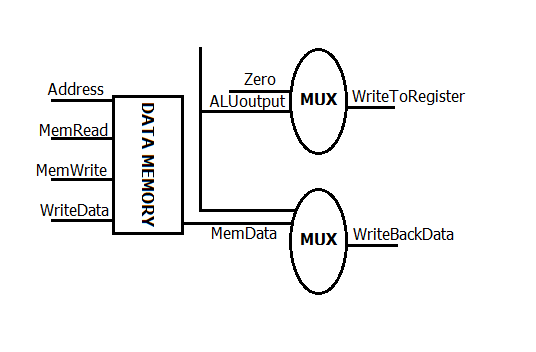
\includegraphics{./datapath/Step4_e_Step5.png}
		\caption*{Datapath dos estágios 4 e 5.}
		\end{center}
	\end{figure}
	\newpage
	
	\begin{landscape}
	\section{Datapath Externo}
	\begin{figure}[H]
    	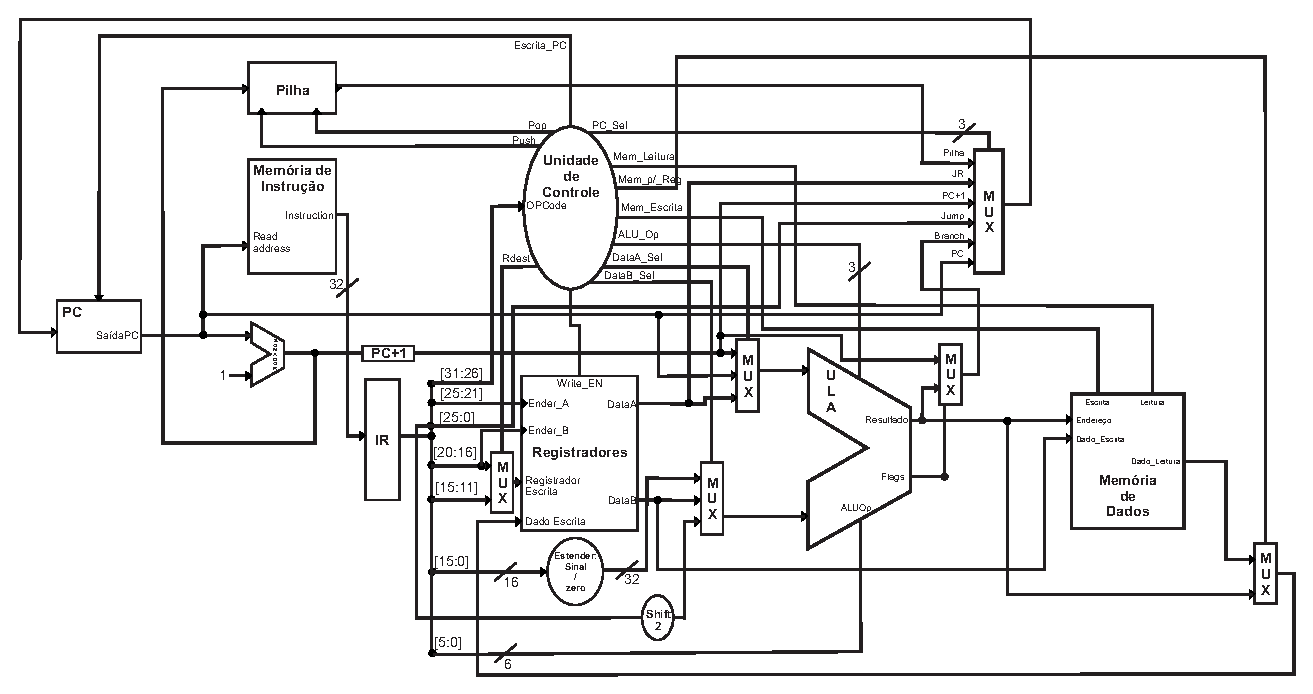
\includegraphics{./datapath/datapath_final-1.eps}
  	\end{figure}
  	\end{landscape}

% Optional bibliography section
% To use bibliograpy, first provide the ipprocess.bib file on the root folder.
% \bibliographystyle{ieeetr}
% \bibliography{ipprocess}

\end{document}